\chapter{Inverse of Matrices}

\section{Left Inverse, Right Inverse, Inverse}

\begin{definition}[$A$的左逆]
    当一个矩阵X满足 $$ X A=I $$ 
    
    X被称为 $ A $ 的\textit{左逆}; 当左逆存在时,则称A是\textit{可左逆}的;
\end{definition}

    如果左逆矩阵存在, 则左逆矩阵有\textbf{无穷多}个.

\begin{example}
    $$ A=\left[\begin{array}{cc}-3 & -4 \\ 4 & 6 \\ 1 & 1\end{array}\right] $$

    矩阵$A$是可左逆的,其左逆矩阵有两个

    $$ B=\frac{1}{9}\left[\begin{array}{ccc}-11 & -10 & 16 \\ 7 & 8 & -11\end{array}\right] \quad C=\frac{1}{2}\left[\begin{array}{ccc}0 & -1 & 6 \\ 0 & 1 & -4\end{array}\right] $$
\end{example}

\begin{definition}[$A$的右逆]
    当左逆存在时,则称A是可左逆的;
\end{definition}

    如果右逆矩阵存在, 则右逆矩阵有\textbf{无穷多}个.


\begin{example}
    $$ B=\left[\begin{array}{lll}1 & 0 & 1 \\ 0 & 1 & 1\end{array}\right] $$

    矩阵$B$可右逆,以下矩阵都是$B$的右逆

    $$ D=\frac{1}{2}\left[\begin{array}{cc}1 & -1 \\ -1 & 1 \\ 1 & 1\end{array}\right], E=\left[\begin{array}{ll}1 & 0 \\ 0 & 1 \\ 0 & 0\end{array}\right], G=\left[\begin{array}{cc}1 & -1 \\ 0 & 0 \\ 0 & 1\end{array}\right] $$
\end{example}

\begin{theorem}
一个大小为 $ m \times n $ 的矩阵, 其左逆或右逆的维度为 $ n \times m $.
\end{theorem}


\begin{theorem}
    A的左逆为 $ X $ 当且仅当 $ X^{T} $ 是 $ A^{T} $ 的右逆.
\end{theorem}

\begin{proof}
    $$
A^{T} X^{T}=(X A)^{T}=I
$$
\end{proof}

\begin{theorem}
    A的右逆为 $ X $ 当且仅当 $ X^{T} $ 是 $ A^{T} $ 的左逆.
\end{theorem}

\begin{proof}
    $$
X^{T} A^{T}=(A X)^{\mathrm{T}}=I
$$
\end{proof}

\begin{theorem}
    如果矩阵A存在左逆和右逆,则左逆和右逆一定相等
\end{theorem}

\begin{proof}
    $$
    \begin{aligned}
    &X A=I, A Y=I  \\
    \Rightarrow&  X=X I=X(A Y)=(X A) Y=Y \\
    \Rightarrow& X=Y
    \end{aligned}
$$
\end{proof}

\begin{definition}[逆 $A^{-1}$]
    如果矩阵A存在左逆和右逆, 此时X称为矩阵的\textit{逆},记作 $ A^{-1} $ 当矩阵的逆存在时,则称矩阵A\textit{可逆}.
\end{definition}

\section{Linear Equation Systems}

\begin{definition}[Linear Equation Systems]
    有$n$个变量的$m$个方程为

    $$ \left\{\begin{array}{c}A_{11} x_{1}+A_{12} x_{2}+\cdots+A_{1 n} x_{n}=b_{1} \\ A_{21} x_{1}+A_{22} x_{2}+\cdots+A_{2 n} x_{n}=b_{2} \\ \vdots \\ A_{m 1} x_{1}+A_{m 2} x_{2}+\cdots+A_{m n} x_{n}=b_{m}\end{array}\right. $$

    写成矩阵形式为: $ \mathrm{A} x=\mathrm{b} $ . 其中$A$为系数矩阵, $ x $ 为$n$维列向量. 
\end{definition}

该方程组可能\textbf{无解},\textbf{有唯一解}和\textbf{无穷解}.

\subsection{线性方程组求解}

\begin{theorem}
    如果矩阵$A$可左逆,假设 $ X $ 是矩阵$A$的左逆,则\textbf{至多}一个解, 如有解则 $ x=X b $ . 
\end{theorem}

\begin{proof}
    $$
A x=b \Rightarrow  x=X A x=X b
$$

    列满秩时(下面证明), 列向量线性无关, 所以其零空间中只有零解,方程 $ {Ax}={b} $ 可能有一个唯一解 ($b$在$A$的列空间中, 此特解就是全部解, 因为通常的特解可以通过零空间中的向量扩展出一组解集,而此时零空间只有$0$向量), 也可能无解 ($b$不在$A$的列空间中). 
\end{proof}

\begin{theorem}
    如果矩阵$A$可右逆,假设 $ Y $ 是矩阵$A$的右逆,则\textbf{至少}一个解, 即 $ x=\mathrm{Y} b $ . 
\end{theorem}

\begin{proof}
    设$x=Y b$ 

    $$
x=Y b  \Rightarrow  A x=A Y b=b
$$


右逆就是研究 $m \times n $ 矩阵$A$行满秩的情况, 此时 $ \mathrm{n}>\mathrm{m}=\operatorname{rank}(\mathrm{A}) $ . 对称的, 其左零空间中仅有零向量,即没有行向量的线性组合能够得到零向量. ($N(A ^T ) = \{0\}$)
\end{proof}

\begin{theorem}
    如果矩阵$A$可逆的,假设 $ X $ 是矩阵$A$的逆,则
$$
A x=b  \Rightarrow  x=A^{-1} b
$$
唯一解. 
\end{theorem}

\section{Fundamental Theorem of Linear Algebra}

\begin{FigureCenter}{Four Subspace of Matrix $A$}
    \tikzset{every picture/.style={line width=0.75pt}} %set default line width to 0.75pt        
    % \resizebox{\textwidth}{!}{%
    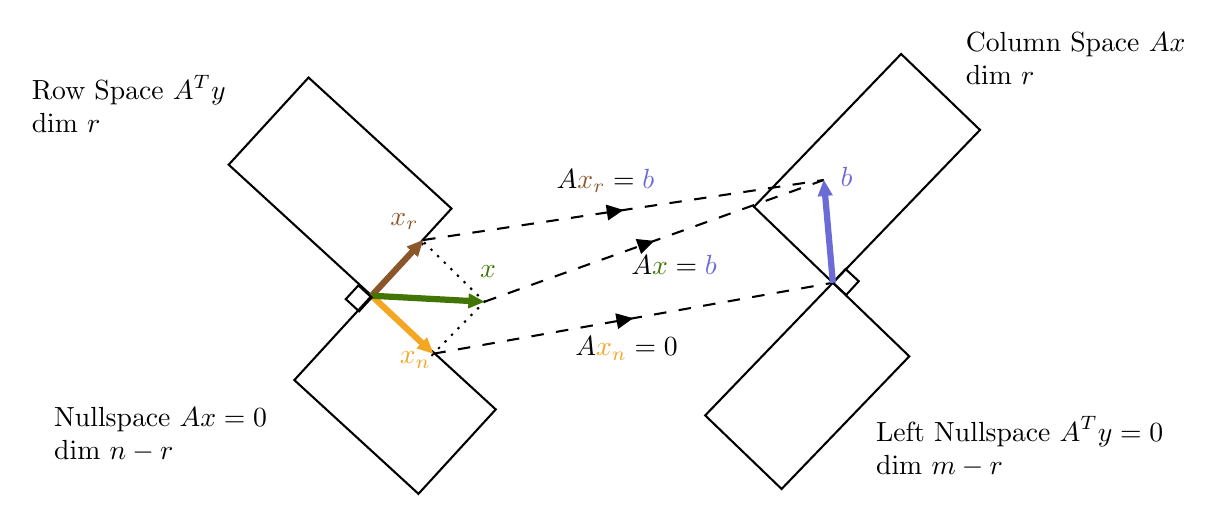
\begin{tikzpicture}[x=0.75pt,y=0.75pt,yscale=-0.9,xscale=0.9]
    
    %\begin{adjustbox}{width=\textwidth}
    %\begin{tikzpicture}   
    %uncomment if require: \path (0,300); %set diagram left start at 0, and has height of 300
    
    %Shape: Rectangle [id:dp8564537788335302] 
    \draw  [dash pattern={on 0.84pt off 2.51pt}] (221.63,153.4) -- (253.96,185.17) -- (225.93,213.7) -- (193.59,181.93) -- cycle ;
    %Shape: Rectangle [id:dp7748103688398633] 
    \draw   (159.81,65.14) -- (236.34,135.27) -- (193.59,181.93) -- (117.06,111.79) -- cycle ;
    %Shape: Rectangle [id:dp3534850306924755] 
    \draw   (193.59,181.93) -- (260.03,242.81) -- (218.64,287.99) -- (152.2,227.1) -- cycle ;
    
    %Shape: Rectangle [id:dp11468847928918202] 
    \draw   (477.03,52.53) -- (398.27,134.34) -- (440.51,175) -- (519.26,93.19) -- cycle ;
    %Shape: Rectangle [id:dp8320016424104848] 
    \draw   (440.51,175) -- (372.14,246.02) -- (413.05,285.39) -- (481.41,214.38) -- cycle ;
    
    %Straight Lines [id:da413550032058265] 
    \draw [color={rgb, 255:red, 139; green, 87; blue, 42 }  ,draw opacity=1 ][line width=2.25]    (193.59,181.93) -- (217.74,155.81) ;
    \draw [shift={(221.14,152.14)}, rotate = 492.75] [fill={rgb, 255:red, 139; green, 87; blue, 42 }  ,fill opacity=1 ][line width=0.08]  [draw opacity=0] (8.57,-4.12) -- (0,0) -- (8.57,4.12) -- cycle    ;
    %Straight Lines [id:da05215716031511208] 
    \draw [color={rgb, 255:red, 245; green, 166; blue, 35 }  ,draw opacity=1 ][line width=2.25]    (193.59,181.93) -- (222.99,209.56) ;
    \draw [shift={(226.64,212.99)}, rotate = 223.23] [fill={rgb, 255:red, 245; green, 166; blue, 35 }  ,fill opacity=1 ][line width=0.08]  [draw opacity=0] (8.57,-4.12) -- (0,0) -- (8.57,4.12) -- cycle    ;
    %Straight Lines [id:da20598638562684246] 
    \draw [color={rgb, 255:red, 65; green, 117; blue, 5 }  ,draw opacity=1 ][line width=2.25]    (193.59,181.93) -- (248.97,184.9) ;
    \draw [shift={(253.96,185.17)}, rotate = 183.08] [fill={rgb, 255:red, 65; green, 117; blue, 5 }  ,fill opacity=1 ][line width=0.08]  [draw opacity=0] (8.57,-4.12) -- (0,0) -- (8.57,4.12) -- cycle    ;
    %Straight Lines [id:da9574000480451021] 
    \draw  [dash pattern={on 4.5pt off 4.5pt}]  (221.14,152.14) -- (435.64,119.99) ;
    \draw [shift={(328.39,136.06)}, rotate = 531.48] [fill={rgb, 255:red, 0; green, 0; blue, 0 }  ][line width=0.08]  [draw opacity=0] (8.93,-4.29) -- (0,0) -- (8.93,4.29) -- cycle    ;
    %Straight Lines [id:da8574440156945131] 
    \draw  [dash pattern={on 4.5pt off 4.5pt}]  (253.96,185.17) -- (435.64,119.99) ;
    \draw [shift={(344.8,152.58)}, rotate = 520.26] [fill={rgb, 255:red, 0; green, 0; blue, 0 }  ][line width=0.08]  [draw opacity=0] (8.93,-4.29) -- (0,0) -- (8.93,4.29) -- cycle    ;
    %Straight Lines [id:da26442247252775863] 
    \draw  [dash pattern={on 4.5pt off 4.5pt}]  (226.64,212.99) -- (440.51,175) ;
    \draw [shift={(333.57,193.99)}, rotate = 529.9300000000001] [fill={rgb, 255:red, 0; green, 0; blue, 0 }  ][line width=0.08]  [draw opacity=0] (8.93,-4.29) -- (0,0) -- (8.93,4.29) -- cycle    ;
    %Shape: Rectangle [id:dp41111107193098295] 
    \draw   (186.5,176.41) -- (193.59,182.93) -- (186.84,190.28) -- (179.74,183.76) -- cycle ;
    %Shape: Rectangle [id:dp37902094791189933] 
    \draw   (447.27,167.65) -- (454.36,174.17) -- (447.61,181.52) -- (440.51,175) -- cycle ;
    %Straight Lines [id:da3897829543263125] 
    \draw [color={rgb, 255:red, 108; green, 108; blue, 215 }  ,draw opacity=1 ][line width=2.25]    (440.51,175) -- (436.08,124.97) ;
    \draw [shift={(435.64,119.99)}, rotate = 444.94] [fill={rgb, 255:red, 108; green, 108; blue, 215 }  ,fill opacity=1 ][line width=0.08]  [draw opacity=0] (8.57,-4.12) -- (0,0) -- (8.57,4.12) -- cycle    ;
    
    % Text Node
    \draw (10,62) node [anchor=north west][inner sep=0.75pt]   [align=left] {Row Space $\displaystyle A^{T} y$\\dim $\displaystyle r$};
    % Text Node
    \draw (22,240) node [anchor=north west][inner sep=0.75pt]   [align=left] {Nullspace $\displaystyle Ax=0$\\dim $\displaystyle n-r$};
    % Text Node
    \draw (510,39) node [anchor=north west][inner sep=0.75pt]   [align=left] {Column Space $\displaystyle Ax$\\dim $\displaystyle r$};
    % Text Node
    \draw (462,245) node [anchor=north west][inner sep=0.75pt]   [align=left] {Left Nullspace $\displaystyle A^{T} y=0$\\dim $\displaystyle m-r$};
    % Text Node
    \draw (291,112.4) node [anchor=north west][inner sep=0.75pt]    {$A\textcolor[rgb]{0.55,0.34,0.16}{x_{r}} =\textcolor[rgb]{0.42,0.42,0.84}{b}$};
    % Text Node
    \draw (202,136.4) node [anchor=north west][inner sep=0.75pt]  [color={rgb, 255:red, 139; green, 87; blue, 42 }  ,opacity=1 ]  {$x_{r}$};
    % Text Node
    \draw (207,210.4) node [anchor=north west][inner sep=0.75pt]  [color={rgb, 255:red, 245; green, 166; blue, 35 }  ,opacity=1 ]  {$x_{n}$};
    % Text Node
    \draw (443,111.4) node [anchor=north west][inner sep=0.75pt]  [color={rgb, 255:red, 108; green, 108; blue, 215 }  ,opacity=1 ]  {$b$};
    % Text Node
    \draw (331,158.4) node [anchor=north west][inner sep=0.75pt]    {$A\textcolor[rgb]{0.25,0.46,0.02}{x} =\textcolor[rgb]{0.42,0.42,0.84}{b}$};
    % Text Node
    \draw (301,202.4) node [anchor=north west][inner sep=0.75pt]    {$A\textcolor[rgb]{0.96,0.65,0.14}{x_{n}} =0$};
    % Text Node
    \draw (250,164.4) node [anchor=north west][inner sep=0.75pt]  [color={rgb, 255:red, 65; green, 117; blue, 5 }  ,opacity=1 ]  {$x$};
    
    \end{tikzpicture}
\end{FigureCenter}





\begin{table}[htbp]
    \begin{tabular}{llll}
    $ \boldsymbol{r}=\boldsymbol{m}  $ & $  \boldsymbol{r}=\boldsymbol{n}  $  & Square and invertible & $  A \boldsymbol{x}=\boldsymbol{b}  $ has 1 solution \\
    $ \boldsymbol{r}=\boldsymbol{m}  $  &  $  r<n  $ &  Short and wide&  $  A \boldsymbol{x}=\boldsymbol{b}  $ has $ \infty $ solutions \\
    $ r<m  $ & $  \boldsymbol{r}=\boldsymbol{n}  $ &   Tall and thin& $  A \boldsymbol{x}=\boldsymbol{b}  $ has 0 or 1 solution \\
    $ r<m  $ &  $  r<n  $ & Not full rank &  $  A \boldsymbol{x}=\boldsymbol{b}  $ has 0 or $ \infty $ solutions
    \end{tabular}
    \end{table}

    The set
    of linear equations is called \term{over-determined} if $ m>n $,  \term{under-determined} if $m \leq n$, and \term{square} if $m = n$.

    A set of equations with zero right-hand side, $ A x=0 $, is called a \term{homogeneous} set of equations. Any homogeneous set of equations has $ x=0 $ as a solution.

\section{Invertible Matrices}

\begin{theorem}
    对于方阵 $ A \in \mathbb{R}^{n \times n} $ ,以下条件都是等价的:

    \begin{enumerate}
        \item $ A $ 可左逆
        \item $A$的列向量线性无关
        \item $A$可右逆
        \item $A$的行向量线性无关
        \item $A$可逆
    \end{enumerate}

    此时矩阵$A$为非奇异矩阵,由条件1与3,可得$A$为可逆矩阵. 
\end{theorem}

\begin{proof}
    可以通过以下方式证明:

    \centering
    \tikzset{every picture/.style={line width=0.75pt}} %set default line width to 0.75pt        

    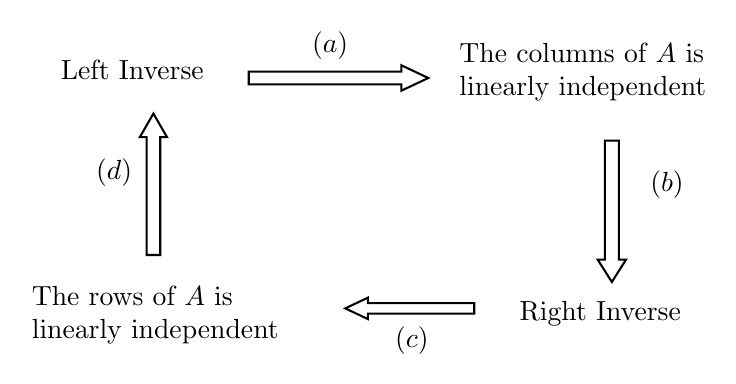
\begin{tikzpicture}[x=0.75pt,y=0.75pt,yscale=-1,xscale=1]
    %uncomment if require: \path (0,300); %set diagram left start at 0, and has height of 300

    %Right Arrow [id:dp1873650424277289] 
    \draw   (269,87.07) -- (342.52,87.07) -- (342.52,84) -- (355.52,90.14) -- (342.52,96.27) -- (342.52,93.2) -- (269,93.2) -- cycle ;
    %Right Arrow [id:dp6482140902579632] 
    \draw   (219.8,175.44) -- (219.8,118.66) -- (216.53,118.66) -- (223.08,107.27) -- (229.64,118.66) -- (226.36,118.66) -- (226.36,175.44) -- cycle ;
    %Right Arrow [id:dp31978358236465754] 
    \draw   (447.37,120.34) -- (447.37,177.66) -- (450.78,177.66) -- (443.96,188.43) -- (437.14,177.66) -- (440.55,177.66) -- (440.55,120.34) -- cycle ;
    %Right Arrow [id:dp9972986143574651] 
    \draw   (377.64,198.57) -- (326.37,198.57) -- (326.37,196) -- (315.52,201.14) -- (326.37,206.27) -- (326.37,203.7) -- (377.64,203.7) -- cycle ;

    % Text Node
    \draw (177,80) node [anchor=north west][inner sep=0.75pt]   [align=left] {Left Inverse};
    % Text Node
    \draw (369,72) node [anchor=north west][inner sep=0.75pt]   [align=left] {The columns of $A$ is\\ linearly independent};
    % Text Node
    \draw (163,189) node [anchor=north west][inner sep=0.75pt]   [align=left] {The rows of $A$ is\\ linearly independent};
    % Text Node
    \draw (398,196) node [anchor=north west][inner sep=0.75pt]   [align=left] {Right Inverse};
    % Text Node
    \draw (298,66.4) node [anchor=north west][inner sep=0.75pt]    {$( a)$};
    % Text Node
    \draw (338,208.4) node [anchor=north west][inner sep=0.75pt]    {$( c)$};
    % Text Node
    \draw (461,133.4) node [anchor=north west][inner sep=0.75pt]    {$( b)$};
    % Text Node
    \draw (194,127.4) node [anchor=north west][inner sep=0.75pt]    {$( d)$};


    \end{tikzpicture}

    \begin{itemize}
        \item 性质 $ (\mathrm{a}) $ 对任意矩阵 $ A \in \mathbb{R}^{m \times n} $ 都成立 
        \item 性质$(b)$对方阵矩阵 $ A \in \mathbb{R}^{n \times n} $ 都成立
        \item 对于性质 $ (\mathrm{c}) $ 与 $ (\mathrm{d}) $, 可利用 $ A^{T} $ 证明
    \end{itemize}
\end{proof}

\begin{theorem}
    $(a)$: $A$可左逆,则$A$列向量线性无关.
\end{theorem}

\begin{proof}
    假设$A$的左逆是 $ B $ ,则
    $$
    \begin{aligned}
            & A x=0 \\
     \Rightarrow &B A x=0 \\
    \Rightarrow & I x=0
    \end{aligned}
    $$

    假设A的列向量 $ A=\left[a_{1}, a_{2}, \cdots, a_{n}\right] $
    $$
    A x=x_{1} a_{1}+x_{2} a_{2}+\cdots+x_{n} a_{n}=0
    $$

    则当该等式 $ A x=0 $ 成立时,其解 $ x=0 $, 则A的列向量线性无关.  
    
    \begin{corollary}
        如果 $ A \in \mathbb{R}^{m \times n} $有左逆,则有 $ m \geq n = r $. 

    即$A$是高或方的矩阵, 如 $ A=\left[\begin{array}{ll}1 & 0 \\ 0 & 1 \\ 0 & 0\end{array}\right] $. 
    
    此时$A$的行向量可能线性相关,而$A$的列向量线性无关. $N(A) = \{0\}$.
    \end{corollary}
    

    假设 $ A $ 的列向量 $ A=\left[a_{1}, a_{2}, \cdots, a_{n}\right] $
    $$
    \begin{aligned}
         A x&=x_{1} a_{1}+x_{2} a_{2}+\cdots+x_{n} a_{n}=b \\
    A y&=y_{1} a_{1}+y_{2} a_{2}+\cdots+y_{n} a_{n}=b \\
    \end{aligned}
    $$

    $$A x-A y=A(x-y)=0 \Rightarrow x=y$$

    当 $ b \in \mathbb{R}^{m}, b \notin\left\{y \mid y=A x, x \in \mathbb{R}^{n}\right\} $ 时(即$b$不在$A$的列空间,$ m \geq n  $时),线性方程组无解.  $ A x=b $ 至多一个解,如有解则 $ x=X b $ . 
\end{proof}

\begin{theorem}
    矩阵的行秩等于列秩.
\end{theorem}

\begin{proof}
    令 $A$ 是一个 $m\times n$ 的矩阵,其列秩为 $r $. 因此矩阵 $A$ 的列空间的维度是 $r$ . 
    
    令 $c_1,c_2,\ldots,c_r$ 是 $A$ 的列空间的一组基,构成 $m \times r$ 矩阵 $C$ 的列向量 $C = [c_1,c_2,\ldots,c_r]$,并使得 $A$ 的每个列向量是 $C$ 的 $r$ 个列向量的线性组合. 
    
    由矩阵乘法的定义,存在一个 $r \times n$ 矩阵 $R$, 使得 $A = CR$. ($A$ 的 $(i,j)$ 元素是 $c_i$ 与 $R$ 的第 $j$ 个行向量的点积.)

现在,由于 $A = CR$, $A$ 的每个行向量是 $R$ 的行向量的线性组合,这意味着 $A$ 的行向量空间被包含于 $R$ 的行向量空间之中. 因此 $A 的行秩 \leq R的行秩$. 但$R$仅有$r$行, 所以$R的行秩 \leq r = A的列秩$. 这就证明了$A的行秩 \leq A的列秩$.

把上述证明过程中的“行”与“列”交换,利用对偶性质同样可证$A的列秩 \leq A的行秩$. 更简单的方法是考虑A的转置矩阵 $A^\mathrm{T}$,则$A的列秩 =  A^\mathrm{T}的行秩 \leq  A^\mathrm{T}的列秩 = A的行秩$. 这证明了$A$的列秩等于$A$的行秩. 证毕.
\end{proof}

\begin{theorem}
    $(c)$: 矩阵 $ A \in \mathbb{R}^{m \times n} $ 有右逆 $ X $, 则A行向量线性无关.
\end{theorem}

\begin{proof}
    $$ \mathrm{X}^{T} A^{T}=(A X)^{T}=I $$
    
    则有 $ \mathrm{X}^{T} $ 是 $ A^{T} $ 的左逆, $ A^{T} $ 的列向量线性无关.  

    即 $ A^{T} \in \mathbb{R}^{n \times m} $.
    
    \begin{corollary}
     如果 $ A \in \mathbb{R}^{m \times n} $有左逆,则有 $r= m \leq n  $. 

    即$A$是宽或方的矩阵. 

    此时$A$的列向量可能线性相关,而$A$的行向量线性无关. 
    
    $N(A^T) = \{0\}, \operatorname{dim} N(A) = n-r, r=m$. ($Ax=b$有无穷解) 
    \end{corollary}
    
    根据定理“矩阵的行秩等于列秩”,$ A^{T} $ 的列向量线性无关,则矩阵 $ A $ 有$m$个线性无关列向量(行向量),即通过 Gram-Schmidt 正交化可得$m$个正交基. 

    $ \forall b \in \mathbb{R}^{m} $, 有 $ b \in\left\{y \mid y=A x, x \in \mathbb{R}^{n}\right\} (m \leq n ) $, 方程 $ A x=b $ 有解,其解为 $ x=X b $ . 
\end{proof}

\begin{theorem}
    $(b)$: 若方阵A列向量线性无关,则A可右逆. 
\end{theorem}

\begin{proof}
    假设 $ A \in \mathbb{R}^{n \times n} $ 为方阵且列向量线性无关 
    
    $$ A=\left[a_{1}, a_{2}, \cdots, a_{n}\right] $$

    则对于任意向量 $ \mathrm{b} \in \mathbb{R}^{n} $, 则向量组 $ \left[a_{1}, a_{2}, \ldots, a_{n}, \mathrm{~b}\right] $ 线性相关,存 在不全为0的系数,使得以下等式成立
    $$
    x_{1} a_{1}+x_{2} a_{2}+\cdots+x_{n} a_{n}+x_{n+1} b=0
    $$

    因为$A$列向量线性无关,则 $ x_{n+1} \neq 0 $(假设$ x_{n+1} = 0 $会推出违反线性无关假设的结论), 即$b$是$A$列向量的线性组合;
    $$
    b=-\frac{x_{1}}{x_{n+1}} a_{1}-\frac{x_{2}}{x_{n+1}} a_{2}-\cdots-\frac{x_{n}}{x_{n+1}} a_{n}
    $$

    存在向量 $ c_{1}, \ldots, c_{n} \in \mathbb{R}^{n} $,使得 
    $$
    \begin{aligned}
        Ac _{1}&=e_{1}\\
         A c_{2}&=e_{2}\\
          \ldots \\
          A c_{n}&=e_{n}
    \end{aligned}
    $$

    则矩阵 $ C=\left[c_{1} c_{2} \ldots c_{n}\right] $ 是矩阵 $ A $ 的右逆, $ A C=I $.

\end{proof}

\section{转置和共轭转置的逆}

\begin{theorem}[转置 $ A^{T} $ 和共轭转置 $ A^{\mathrm{H}} $ ]
    如果矩阵$A$为非奇异矩阵,则其转置 $ A^{T} $ 和共轭转置 $ A^{\mathrm{H}} $ 都为非奇异矩阵,则有
$$
\begin{array}{l}
\left(A^{T}\right)^{-1}=\left(A^{-1}\right)^{T}, \quad\left(A^{H}\right)^{-1}=\left(A^{-1}\right)^{H} \\
\end{array}
$$
\end{theorem}

\begin{proof}
    $$\left(A A^{-1}\right)^{T}=I \Rightarrow \underbrace{\left(A^{-1}\right)^{T}}_{\text{the inverse of }A^T}   A^{T}=I$$
\end{proof}

\begin{corollary}
    如果矩阵A和矩阵B都为非奇异矩阵,则乘积AB也为非 奇异矩阵
$$
\begin{array}{l}
(A B)^{-1}=B^{-1} A^{-1} \\
\end{array}
$$
\end{corollary}

\begin{proof}
    $$(A B) \underbrace{B^{-1} A^{-1}} _{\text{the inverse of AB}}=I$$
\end{proof}

\section{Gram Matrix非奇异的性质}

\label{Sect:GramNonSingular}

Gram矩阵的定义见 \ref{Def:Gram}.

\begin{corollary}[Gram Matrix 可逆等价于$A$列线性无关]
    矩阵 $ A \in \mathbb{R}^{m \times n},  \mathrm{G}=A^{T} A $

矩阵 $ A $ 列向量线性无关 $ \Leftrightarrow $ Gram矩阵G非奇异.
\end{corollary}

\begin{proof}
    " $ \Rightarrow $ ": 
    
    假设矩阵 $ A $ 列向量线性无关, $ A^{T} A $ 奇异.  则存在 $ A^{T} A x=0, x \neq 0 $, 可得 $ x^{T} A^{T} A x=\|A x\|_{2}^{2}=0 $, 即 $ A x=0 $ 与列向量线性无矛盾.

    " $ \Leftarrow $ ":
    
    假设 $ A^{T} A $ 非奇异, 矩阵 $ A $ 列向量线性相关.  则有 $ A x=0, x \neq 0 $, 可得 $ A^{T} A x=0 $, 即 $ A^{T} A $ 是奇异矩阵. 
\end{proof}

\section{伪逆}

\begin{definition}[Pseudo-inverse]
    $$ A^{\dagger}=A^{T}\left(A A^{T}\right)^{-1} $$

    $$A^{\dagger} = V \Sigma^+ U^T = \left[v_{1} \cdots v_{r} \cdots v_{n}\right]\left[\begin{array}{lll}
        \sigma_{1}^{-1} & & \\
        & \ddots & \\
        & & \sigma_{r}^{-1}
        \end{array}\right]\left[u_{1} \cdots u_{r} \cdots u_{m}\right]^{\mathrm{T}}$$
\end{definition}

\begin{theorem}
    伪逆 $ A^{\dagger} $ 为 $ A $ 的右逆
\end{theorem}

\begin{proof}
    $$ A A^{\dagger}=A A^{T}\left(A A^{T}\right)^{-1}=\left(A A^{T}\right)^{-1}\left(A A^{T}\right)=I $$
\end{proof}

\begin{theorem}
    当$A$为方阵时,右逆等于矩阵的逆
\end{theorem}

\begin{proof}
    $$ A^{\dagger}=A^{T}\left(A A^{T}\right)^{-1}=A^{T} A^{-T} A^{-1}=A^{-1} $$
\end{proof}

\begin{theorem}
    
\end{theorem}

\begin{corollary}
    以下三个结论为等价的,对于实矩阵$A$

    \begin{itemize}
        \item $A$是可左逆的
        \item $A$的列向量线性无关
        \item $ A^{T} A $ 为非奇异矩阵
    \end{itemize}
\end{corollary}

\begin{corollary}
    以下三个结论为等价的,对于实矩阵$A$

    \begin{itemize}
        \item $A$是可右逆的 
        \item $A$的行向量线性无关
        \item $ A A^{T} $ 为非奇异矩阵
    \end{itemize}
\end{corollary}

By choosing good bases, $A$ multiplies $\boldsymbol{v}_{i}$ in the row space to give $\sigma_{i} \boldsymbol{u}_{i}$ in the column space. $A^{-1}$ must do the opposite! 



If $A \boldsymbol{v}=\sigma \boldsymbol{u}$ then $A^{-1} \boldsymbol{u}=\boldsymbol{v} / \sigma$. The singular values of $A^{-1}$ are $1 / \sigma$, just as the eigenvalues of $A^{-1}$ are $1 / \lambda$. The bases are reversed. The $u$ 's are in the row space of $A^{-1}$, the $v$ 's are in the column space.

The pseudoinverse $A^{+}$is an $n$ by $m$ matrix. \textbf{If $A^{-1}$ exists, then $A^{+}$is the same as $A^{-1}$}. In that case $m=n=r$ and we are inverting $U \Sigma V^{\mathrm{T}}$ to get $V \Sigma^{-1} U^{\mathrm{T}}$. 

The new symbol $A^{+}$is needed when $r<m$ or $r<n$. Then $A$ has no two-sided inverse, but it has a \textit{pseudo}inverse $A^{+}$with that same rank $r$ :

$$
A^{+} \boldsymbol{u}_{i}=\frac{1}{\sigma_{i}} \boldsymbol{v}_{i} \quad \text { for } i \leq r \quad \text { and } \quad A^{+} \boldsymbol{u}_{i}=\mathbf{0} \quad \text { for } i>r
$$

The vectors $\boldsymbol{u}_{1}, \ldots, \boldsymbol{u}_{r}$ in the column space of $A$ go back to $\boldsymbol{v}_{1}, \ldots, \boldsymbol{v}_{r}$ in the row space.


The other vectors $\boldsymbol{u}_{r+1}, \ldots, \boldsymbol{u}_{m}$ are in the left nullspace, and $A^{+}$sends them to zero. When we know what happens to all those basis vectors, we know $A^{+}$.

Notice the pseudoinverse of the diagonal matrix $\Sigma .$ Each $\sigma$ in $\Sigma$ is replaced by $\sigma^{-1}$ in $\Sigma^{+} .$The product $\Sigma^{+} \Sigma$ is as near to the identity as we can get. It is a projection matrix, $\Sigma^{+} \Sigma$ is partly $I$ and otherwise zero. We can invert the $\sigma$ 's, but we can't do anything about the zero rows and columns. 

\begin{FigureCenter}{$ A \boldsymbol{x}^{\dagger} $ in the column space goes back to $ A^{\dagger} A \boldsymbol{x}^{\dagger}=\boldsymbol{x}^{\dagger}$ in the row space}
    

    \tikzset{every picture/.style={line width=0.75pt}} %set default line width to 0.75pt        
    
    \begin{tikzpicture}[x=0.75pt,y=0.75pt,yscale=-1,xscale=1]
    %uncomment if require: \path (0,457); %set diagram left start at 0, and has height of 457
    
    %Shape: Rectangle [id:dp8596899930926358] 
    \draw  [dash pattern={on 0.84pt off 2.51pt}] (412.64,146.65) -- (440.94,174.46) -- (412.24,203.67) -- (383.93,175.86) -- cycle ;
    %Shape: Rectangle [id:dp144129295466213] 
    \draw   (159.81,65.14) -- (236.34,135.27) -- (193.59,181.93) -- (117.06,111.79) -- cycle ;
    %Shape: Rectangle [id:dp4244539260616451] 
    \draw   (193.59,181.93) -- (260.03,242.81) -- (218.64,287.99) -- (152.2,227.1) -- cycle ;
    
    %Shape: Rectangle [id:dp10811540545272225] 
    \draw   (477.03,51.53) -- (398.27,133.34) -- (440.51,174) -- (519.26,92.19) -- cycle ;
    %Shape: Rectangle [id:dp952165170642489] 
    \draw   (440.51,174) -- (372.14,245.02) -- (413.05,284.39) -- (481.41,213.38) -- cycle ;
    
    %Straight Lines [id:da43480021093829335] 
    \draw [color={rgb, 255:red, 139; green, 87; blue, 42 }  ,draw opacity=1 ][line width=2.25]    (193.59,181.93) -- (187.34,138.27) ;
    \draw [shift={(186.64,133.33)}, rotate = 441.85] [fill={rgb, 255:red, 139; green, 87; blue, 42 }  ,fill opacity=1 ][line width=0.08]  [draw opacity=0] (8.57,-4.12) -- (0,0) -- (8.57,4.12) -- cycle    ;
    %Straight Lines [id:da6356667569876433] 
    \draw [color={rgb, 255:red, 245; green, 166; blue, 35 }  ,draw opacity=1 ][line width=2.25]    (440.51,175) -- (415.75,200.11) ;
    \draw [shift={(412.24,203.67)}, rotate = 314.6] [fill={rgb, 255:red, 245; green, 166; blue, 35 }  ,fill opacity=1 ][line width=0.08]  [draw opacity=0] (8.57,-4.12) -- (0,0) -- (8.57,4.12) -- cycle    ;
    %Straight Lines [id:da22563123154133025] 
    \draw [color={rgb, 255:red, 65; green, 117; blue, 5 }  ,draw opacity=1 ][line width=2.25]    (440.51,175) -- (388.93,175.78) ;
    \draw [shift={(383.93,175.86)}, rotate = 359.13] [fill={rgb, 255:red, 65; green, 117; blue, 5 }  ,fill opacity=1 ][line width=0.08]  [draw opacity=0] (8.57,-4.12) -- (0,0) -- (8.57,4.12) -- cycle    ;
    %Shape: Rectangle [id:dp12172823301153524] 
    \draw   (186.5,176.41) -- (193.59,182.93) -- (186.84,190.28) -- (179.74,183.76) -- cycle ;
    %Shape: Rectangle [id:dp9349834759264539] 
    \draw   (447.27,167.65) -- (454.36,174.17) -- (447.61,181.52) -- (440.51,175) -- cycle ;
    %Straight Lines [id:da2510398254796229] 
    \draw [color={rgb, 255:red, 108; green, 108; blue, 215 }  ,draw opacity=1 ][line width=2.25]    (440.51,175) -- (416.14,150.21) ;
    \draw [shift={(412.64,146.65)}, rotate = 405.49] [fill={rgb, 255:red, 108; green, 108; blue, 215 }  ,fill opacity=1 ][line width=0.08]  [draw opacity=0] (8.57,-4.12) -- (0,0) -- (8.57,4.12) -- cycle    ;
    %Straight Lines [id:da5471202445204062] 
    \draw  [dash pattern={on 4.5pt off 4.5pt}]  (383.93,175.86) -- (186.64,133.33) ;
    \draw [shift={(285.28,154.59)}, rotate = 372.15999999999997] [fill={rgb, 255:red, 0; green, 0; blue, 0 }  ][line width=0.08]  [draw opacity=0] (8.93,-4.29) -- (0,0) -- (8.93,4.29) -- cycle    ;
    %Straight Lines [id:da12114390650727058] 
    \draw  [dash pattern={on 4.5pt off 4.5pt}]  (412.64,146.65) -- (186.64,133.33) ;
    \draw [shift={(299.64,139.99)}, rotate = 363.37] [fill={rgb, 255:red, 0; green, 0; blue, 0 }  ][line width=0.08]  [draw opacity=0] (8.93,-4.29) -- (0,0) -- (8.93,4.29) -- cycle    ;
    %Straight Lines [id:da8219115744539653] 
    \draw  [dash pattern={on 4.5pt off 4.5pt}]  (412.24,203.67) -- (193.59,181.93) ;
    \draw [shift={(302.92,192.8)}, rotate = 365.68] [fill={rgb, 255:red, 0; green, 0; blue, 0 }  ][line width=0.08]  [draw opacity=0] (8.93,-4.29) -- (0,0) -- (8.93,4.29) -- cycle    ;
    
    % Text Node
    \draw (9,64) node [anchor=north west][inner sep=0.75pt]   [align=left] {Row Space $\displaystyle A^{T} y$\\dim $\displaystyle r$};
    % Text Node
    \draw (16,217) node [anchor=north west][inner sep=0.75pt]   [align=left] {Nullspace $\displaystyle Ax=0$\\dim $\displaystyle n-r$};
    % Text Node
    \draw (506,32) node [anchor=north west][inner sep=0.75pt]   [align=left] {Column Space $\displaystyle Ax$\\dim $\displaystyle r$};
    % Text Node
    \draw (469,224) node [anchor=north west][inner sep=0.75pt]   [align=left] {Left Nullspace $\displaystyle A^{T} y=0$\\dim $\displaystyle m-r$};
    % Text Node
    \draw (173,114.4) node [anchor=north west][inner sep=0.75pt]  [color={rgb, 255:red, 139; green, 87; blue, 42 }  ,opacity=1 ]  {$x^{\dagger }$};
    % Text Node
    \draw (417,202.4) node [anchor=north west][inner sep=0.75pt]  [color={rgb, 255:red, 245; green, 166; blue, 35 }  ,opacity=1 ]  {$e$};
    % Text Node
    \draw (423,132.4) node [anchor=north west][inner sep=0.75pt]  [color={rgb, 255:red, 108; green, 108; blue, 215 }  ,opacity=1 ]  {$p$};
    % Text Node
    \draw (370,167.4) node [anchor=north west][inner sep=0.75pt]  [color={rgb, 255:red, 65; green, 117; blue, 5 }  ,opacity=1 ]  {$b$};
    % Text Node
    \draw (473,153.4) node [anchor=north west][inner sep=0.75pt]  [color={rgb, 255:red, 108; green, 108; blue, 215 }  ,opacity=1 ]  {$ \begin{array}{l}
    \textcolor[rgb]{0.42,0.42,0.84}{p}\textcolor[rgb]{0,0,0}{=A}\textcolor[rgb]{0.55,0.34,0.16}{x}\textcolor[rgb]{0.55,0.34,0.16}{^{\dagger }}\\
    \textcolor[rgb]{0,0,0}{=AA}\textcolor[rgb]{0,0,0}{^{\dagger }}\textcolor[rgb]{0.25,0.46,0.02}{b}\\
    \end{array}$};
    % Text Node
    \draw (276,197.4) node [anchor=north west][inner sep=0.75pt]    {$A^{\dagger } e=0$};
    % Text Node
    \draw (241,160.4) node [anchor=north west][inner sep=0.75pt]    {$A^{\dagger }\textcolor[rgb]{0.25,0.46,0.02}{b} =\textcolor[rgb]{0.55,0.34,0.16}{x}\textcolor[rgb]{0.55,0.34,0.16}{^{\dagger }}$};
    % Text Node
    \draw (287,113.4) node [anchor=north west][inner sep=0.75pt]    {$A^{\dagger }\textcolor[rgb]{0.42,0.42,0.84}{p} =\textcolor[rgb]{0.55,0.34,0.16}{x}\textcolor[rgb]{0.55,0.34,0.16}{^{\dagger }}$};
    % Text Node
    \draw  [color={rgb, 255:red, 0; green, 0; blue, 0 }  ,draw opacity=0 ][fill={rgb, 255:red, 249; green, 192; blue, 139 }  ,fill opacity=1 ][dash pattern={on 0.84pt off 2.51pt}]  (208,43) .. controls (208,40.24) and (210.24,38) .. (213,38) -- (418,38) .. controls (420.76,38) and (423,40.24) .. (423,43) -- (423,83) .. controls (423,85.76) and (420.76,88) .. (418,88) -- (213,88) .. controls (210.24,88) and (208,85.76) .. (208,83) -- cycle  ;
    \draw (211,42.4) node [anchor=north west][inner sep=0.75pt]    {$A^{\dagger } A=\begin{bmatrix}
    I & 0\\
    0 & 0
    \end{bmatrix} \ \begin{matrix}
    (\text{row\ space})\\
    (\text{nullspace})
    \end{matrix}$};
    % Text Node
    \draw (122,133) node [anchor=north west][inner sep=0.75pt]   [align=left] {text};
    % Text Node
    \draw  [color={rgb, 255:red, 0; green, 0; blue, 0 }  ,draw opacity=0 ][fill={rgb, 255:red, 249; green, 192; blue, 139 }  ,fill opacity=1 ]  (191,307) .. controls (191,304.24) and (193.24,302) .. (196,302) -- (443,302) .. controls (445.76,302) and (448,304.24) .. (448,307) -- (448,347) .. controls (448,349.76) and (445.76,352) .. (443,352) -- (196,352) .. controls (193.24,352) and (191,349.76) .. (191,347) -- cycle  ;
    \draw (194,306.4) node [anchor=north west][inner sep=0.75pt]    {$\begin{matrix}
    A & \text{Row\ space\ to\ column\ space}\\
    A^{\dagger } & \text{Column\ space\ to\ row\ space}
    \end{matrix}$};
    
    
    \end{tikzpicture}
    \end{FigureCenter}

\begin{FigureCenter}{Projection from row space to column space}
    

\tikzset{every picture/.style={line width=0.75pt}} %set default line width to 0.75pt        

\begin{tikzpicture}[x=0.75pt,y=0.75pt,yscale=-1,xscale=1]
%uncomment if require: \path (0,376); %set diagram left start at 0, and has height of 376

%Shape: Rectangle [id:dp8564537788335302] 
\draw  [dash pattern={on 0.84pt off 2.51pt}] (221.63,153.4) -- (253.96,185.17) -- (225.93,213.7) -- (193.59,181.93) -- cycle ;
%Shape: Rectangle [id:dp7748103688398633] 
\draw   (159.81,65.14) -- (236.34,135.27) -- (193.59,181.93) -- (117.06,111.79) -- cycle ;
%Shape: Rectangle [id:dp3534850306924755] 
\draw   (193.59,181.93) -- (260.03,242.81) -- (218.64,287.99) -- (152.2,227.1) -- cycle ;

%Shape: Rectangle [id:dp11468847928918202] 
\draw   (477.03,52.53) -- (398.27,134.34) -- (440.51,175) -- (519.26,93.19) -- cycle ;
%Shape: Rectangle [id:dp8320016424104848] 
\draw   (440.51,175) -- (372.14,246.02) -- (413.05,285.39) -- (481.41,214.38) -- cycle ;

%Straight Lines [id:da413550032058265] 
\draw [color={rgb, 255:red, 139; green, 87; blue, 42 }  ,draw opacity=1 ][line width=2.25]    (193.59,181.93) -- (217.74,155.81) ;
\draw [shift={(221.14,152.14)}, rotate = 492.75] [fill={rgb, 255:red, 139; green, 87; blue, 42 }  ,fill opacity=1 ][line width=0.08]  [draw opacity=0] (8.57,-4.12) -- (0,0) -- (8.57,4.12) -- cycle    ;
%Straight Lines [id:da05215716031511208] 
\draw [color={rgb, 255:red, 245; green, 166; blue, 35 }  ,draw opacity=1 ][line width=2.25]    (193.59,181.93) -- (222.99,209.56) ;
\draw [shift={(226.64,212.99)}, rotate = 223.23] [fill={rgb, 255:red, 245; green, 166; blue, 35 }  ,fill opacity=1 ][line width=0.08]  [draw opacity=0] (8.57,-4.12) -- (0,0) -- (8.57,4.12) -- cycle    ;
%Straight Lines [id:da20598638562684246] 
\draw [color={rgb, 255:red, 65; green, 117; blue, 5 }  ,draw opacity=1 ][line width=2.25]    (193.59,181.93) -- (248.97,184.9) ;
\draw [shift={(253.96,185.17)}, rotate = 183.08] [fill={rgb, 255:red, 65; green, 117; blue, 5 }  ,fill opacity=1 ][line width=0.08]  [draw opacity=0] (8.57,-4.12) -- (0,0) -- (8.57,4.12) -- cycle    ;
%Straight Lines [id:da9574000480451021] 
\draw  [dash pattern={on 4.5pt off 4.5pt}]  (221.14,152.14) -- (435.64,119.99) ;
\draw [shift={(328.39,136.06)}, rotate = 531.48] [fill={rgb, 255:red, 0; green, 0; blue, 0 }  ][line width=0.08]  [draw opacity=0] (8.93,-4.29) -- (0,0) -- (8.93,4.29) -- cycle    ;
%Straight Lines [id:da8574440156945131] 
\draw  [dash pattern={on 4.5pt off 4.5pt}]  (253.96,185.17) -- (435.64,119.99) ;
\draw [shift={(344.8,152.58)}, rotate = 520.26] [fill={rgb, 255:red, 0; green, 0; blue, 0 }  ][line width=0.08]  [draw opacity=0] (8.93,-4.29) -- (0,0) -- (8.93,4.29) -- cycle    ;
%Straight Lines [id:da26442247252775863] 
\draw  [dash pattern={on 4.5pt off 4.5pt}]  (226.64,212.99) -- (440.51,175) ;
\draw [shift={(333.57,193.99)}, rotate = 529.9300000000001] [fill={rgb, 255:red, 0; green, 0; blue, 0 }  ][line width=0.08]  [draw opacity=0] (8.93,-4.29) -- (0,0) -- (8.93,4.29) -- cycle    ;
%Shape: Rectangle [id:dp41111107193098295] 
\draw   (186.5,176.41) -- (193.59,182.93) -- (186.84,190.28) -- (179.74,183.76) -- cycle ;
%Shape: Rectangle [id:dp37902094791189933] 
\draw   (447.27,167.65) -- (454.36,174.17) -- (447.61,181.52) -- (440.51,175) -- cycle ;
%Straight Lines [id:da3897829543263125] 
\draw [color={rgb, 255:red, 108; green, 108; blue, 215 }  ,draw opacity=1 ][line width=2.25]    (440.51,175) -- (436.08,124.97) ;
\draw [shift={(435.64,119.99)}, rotate = 444.94] [fill={rgb, 255:red, 108; green, 108; blue, 215 }  ,fill opacity=1 ][line width=0.08]  [draw opacity=0] (8.57,-4.12) -- (0,0) -- (8.57,4.12) -- cycle    ;

% Text Node
\draw (10,62) node [anchor=north west][inner sep=0.75pt]   [align=left] {Row Space $\displaystyle A^{T} y$\\dim $\displaystyle r$};
% Text Node
\draw (22,240) node [anchor=north west][inner sep=0.75pt]   [align=left] {Nullspace $\displaystyle Ax=0$\\dim $\displaystyle n-r$};
% Text Node
\draw (510,39) node [anchor=north west][inner sep=0.75pt]   [align=left] {Column Space $\displaystyle Ax$\\dim $\displaystyle r$};
% Text Node
\draw (462,245) node [anchor=north west][inner sep=0.75pt]   [align=left] {Left Nullspace $\displaystyle A^{T} y=0$\\dim $\displaystyle m-r$};
% Text Node
\draw (291,112.4) node [anchor=north west][inner sep=0.75pt]    {$A\textcolor[rgb]{0.55,0.34,0.16}{x}\textcolor[rgb]{0.55,0.34,0.16}{_{r}} =\textcolor[rgb]{0.42,0.42,0.84}{b}$};
% Text Node
\draw (202,136.4) node [anchor=north west][inner sep=0.75pt]  [color={rgb, 255:red, 139; green, 87; blue, 42 }  ,opacity=1 ]  {$x_{r}$};
% Text Node
\draw (207,210.4) node [anchor=north west][inner sep=0.75pt]  [color={rgb, 255:red, 245; green, 166; blue, 35 }  ,opacity=1 ]  {$x_{n}$};
% Text Node
\draw (443,111.4) node [anchor=north west][inner sep=0.75pt]  [color={rgb, 255:red, 108; green, 108; blue, 215 }  ,opacity=1 ]  {$b$};
% Text Node
\draw (331,158.4) node [anchor=north west][inner sep=0.75pt]    {$A\textcolor[rgb]{0.25,0.46,0.02}{x} =\textcolor[rgb]{0.42,0.42,0.84}{b}$};
% Text Node
\draw (301,202.4) node [anchor=north west][inner sep=0.75pt]    {$A\textcolor[rgb]{0.96,0.65,0.14}{x}\textcolor[rgb]{0.96,0.65,0.14}{_{n}} =0$};
% Text Node
\draw (250,164.4) node [anchor=north west][inner sep=0.75pt]  [color={rgb, 255:red, 65; green, 117; blue, 5 }  ,opacity=1 ]  {$x$};
% Text Node
\draw  [color={rgb, 255:red, 0; green, 0; blue, 0 }  ,draw opacity=0 ][fill={rgb, 255:red, 249; green, 192; blue, 139 }  ,fill opacity=1 ]  (191,305) .. controls (191,302.24) and (193.24,300) .. (196,300) -- (443,300) .. controls (445.76,300) and (448,302.24) .. (448,305) -- (448,345) .. controls (448,347.76) and (445.76,350) .. (443,350) -- (196,350) .. controls (193.24,350) and (191,347.76) .. (191,345) -- cycle  ;
\draw (194,304.4) node [anchor=north west][inner sep=0.75pt]    {$\begin{matrix}
A & \text{Row\ space\ to\ column\ space}\\
A^{\dagger } & \text{Column\ space\ to\ row\ space}
\end{matrix}$};


\end{tikzpicture}
\end{FigureCenter}